% Model overview figure — standalone TikZ
% Compile:  pdflatex fig_model_overview.tex
% Include:  \includegraphics[width=\linewidth]{fig_model_overview.pdf}

\documentclass[tikz,border=2pt]{standalone}
\usepackage{amsmath,amssymb}
\usetikzlibrary{
  arrows.meta,
  positioning,
  calc,
  fit,
  backgrounds,
  shapes.geometric,
  decorations.pathreplacing,
  matrix
}
\usepackage{pgfplots}
\pgfplotsset{compat=1.18}

% ── Color palette (matches PNAS journal figures) ──────────────
\definecolor{rna}{HTML}{3C78D8}      % Steel blue — RNA / qPCR
\definecolor{pfu}{HTML}{CC3333}      % Muted red  — PFU / culture
\definecolor{lfd}{HTML}{6AA84F}      % Sage green — LFD
\definecolor{sym}{HTML}{D4A017}      % Dark gold  — Symptoms
\definecolor{pop}{HTML}{94A3B8}      % Light slate — population params
\definecolor{platecol}{HTML}{CBD5E1} % Very light slate — plate borders
\definecolor{obsbox}{HTML}{E2E8F0}   % Light slate — observed fill
\definecolor{inf}{HTML}{7C3AED}      % Violet — infectiousness

\begin{document}

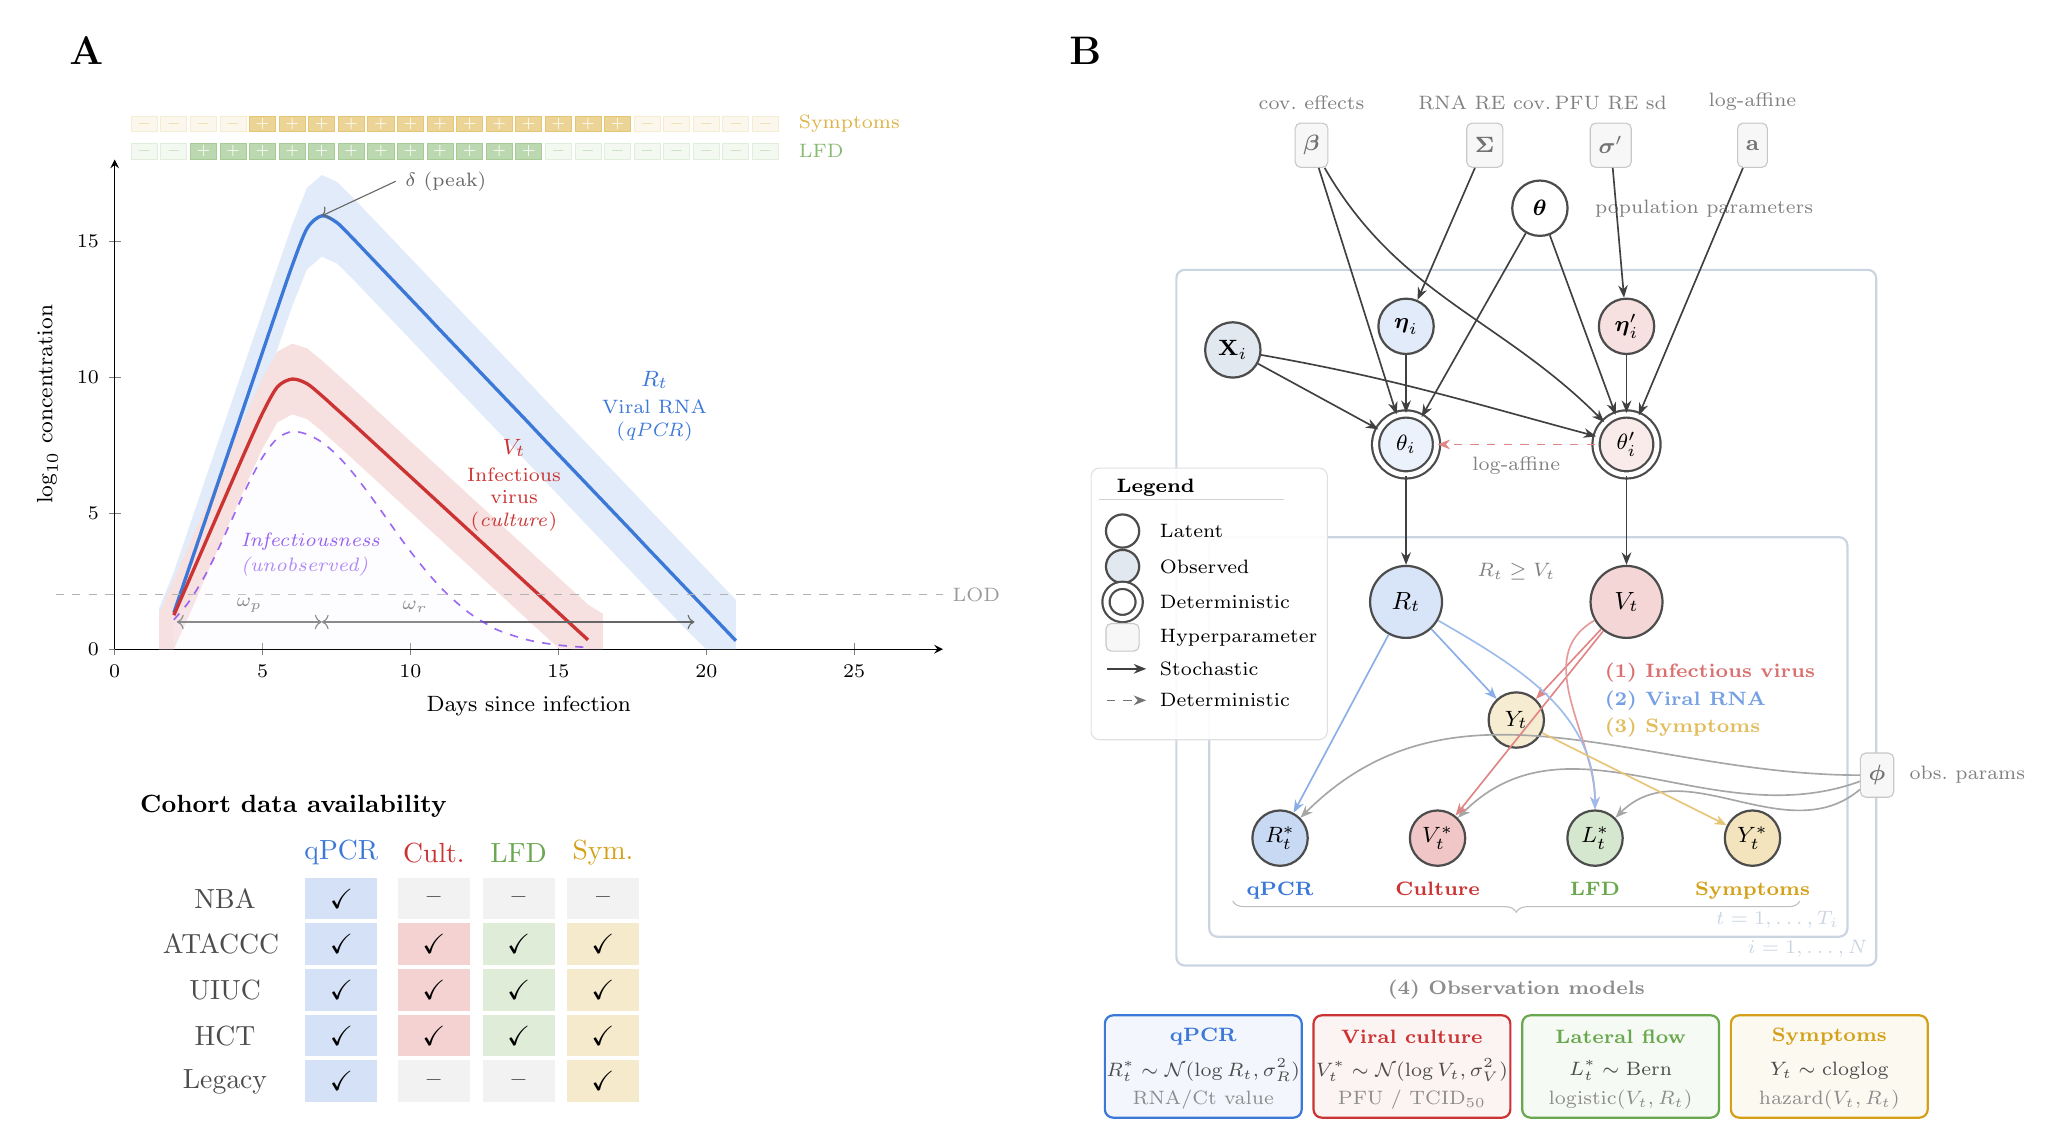
\begin{tikzpicture}[
  % ── Node styles ──
  latent/.style={
    circle, draw=black!70, thick,
    minimum size=20pt, inner sep=1pt, font=\footnotesize
  },
  obs/.style={
    circle, draw=black!70, thick, fill=obsbox,
    minimum size=20pt, inner sep=1pt, font=\footnotesize
  },
  det/.style={
    circle, draw=black!70, thick, double, double distance=1.8pt,
    minimum size=22pt, inner sep=1pt, font=\footnotesize
  },
  hyper/.style={
    draw=black!22, rounded corners=2pt,
    minimum height=16pt, inner sep=3pt,
    font=\footnotesize, fill=black!3, text=black!55
  },
  % ── Arrow styles ──
  to/.style={-{Stealth[length=4.5pt,width=3.5pt]}, semithick, black!75},
  dto/.style={-{Stealth[length=4.5pt,width=3.5pt]}, semithick, dashed, black!55},
  % ── Plate style ──
  plate/.style={
    draw=platecol, thick, rounded corners=3pt,
    inner sep=10pt, fill=none
  },
  plate label/.style={font=\scriptsize\itshape, text=platecol},
  % ── Misc ──
  annot/.style={font=\scriptsize, text=black!50},
  component/.style={font=\scriptsize\bfseries},
]

% ====================================================================
%  PANEL B: PLATE DIAGRAM  (right half)
% ====================================================================
\begin{scope}[shift={(12, 0)}, local bounding box=panelB]

% ── Panel label ──
\node[font=\fontsize{14}{16}\selectfont\bfseries, anchor=north west]
  at (-5.8, 10.3) {B};

% ────────────────────────────────────────────────────
% TOP: Hyperparameters (muted, outside plates)
% ────────────────────────────────────────────────────
\node[hyper] (beta)  at (-2.6, 8.8) {$\boldsymbol{\beta}$};
\node[hyper] (Sigma) at (-0.4, 8.8) {$\boldsymbol{\Sigma}$};
\node[hyper] (spfu)  at (1.2, 8.8)  {$\boldsymbol{\sigma}'$};
\node[hyper] (avec)  at (3.0, 8.8)  {$\mathbf{a}$};

\node[above=1pt of beta,  annot] {cov.\ effects};
\node[above=1pt of Sigma, annot] {RNA RE cov.};
\node[above=1pt of spfu,  annot] {PFU RE sd};
\node[above=1pt of avec,  annot] {log-affine};

% Population kinetic params
\node[latent] (theta) at (0.3, 8) {$\boldsymbol{\theta}$};
\node[annot, anchor=west, xshift=6pt] at (theta.east)
  {population parameters};

% ────────────────────────────────────────────────────
% INDIVIDUAL PLATE
% ────────────────────────────────────────────────────

% Covariates (observed)
\node[obs] (Xi) at (-3.6, 6.2) {$\mathbf{X}_i$};

% Random effects
\node[latent, fill=rna!15] (eta_r) at (-1.4, 6.5) {$\boldsymbol{\eta}_i$};
\node[latent, fill=pfu!15] (eta_p) at (1.4, 6.5)  {$\boldsymbol{\eta}'_i$};

% Individual kinetic params (deterministic nodes)
\node[det, fill=rna!10] (thetaR) at (-1.4, 5) {$\theta_i$};
\node[det, fill=pfu!10] (thetaP) at (1.4, 5)  {$\theta'_i$};

% ────────────────────────────────────────────────────
% TIME PLATE (nested)
% ────────────────────────────────────────────────────

% Latent trajectories (larger, emphasized)
\node[latent, fill=rna!20, minimum size=26pt, font=\small]
  (Rt) at (-1.4, 3) {$R_t$};
\node[latent, fill=pfu!20, minimum size=26pt, font=\small]
  (Vt) at (1.4, 3)  {$V_t$};

% Constraint annotation
\node[annot, anchor=south] at (0, 3.15) {$R_t \geq V_t$};

% Symptom onset
\node[latent, fill=sym!20] (Yt) at (0, 1.5) {$Y_t$};

% Observed measurements
\node[obs, fill=rna!28]  (Rst) at (-3, 0) {$R^*_t$};
\node[obs, fill=pfu!28]  (Vst) at (-1, 0) {$V^*_t$};
\node[obs, fill=lfd!28]  (Lst) at (1, 0)  {$L^*_t$};
\node[obs, fill=sym!28]  (Yst) at (3, 0)  {$Y^*_t$};

% Observation labels
\node[below=2pt of Rst, font=\scriptsize\bfseries, text=rna] (Rst_label)  {qPCR};
\node[below=2pt of Vst, font=\scriptsize\bfseries, text=pfu] (Vst_label)  {Culture};
\node[below=2pt of Lst, font=\scriptsize\bfseries, text=lfd] (Lst_label)  {LFD};
\node[below=2pt of Yst, font=\scriptsize\bfseries, text=sym] (Yst_label)  {Symptoms};

% ── Draw plates ──
% Time plate
\node[plate, fit=(Rt)(Vt)(Yt)(Rst)(Vst)(Lst)(Yst)(Rst_label)(Vst_label)(Lst_label)(Yst_label),
  label={[plate label, anchor=south east]south east:{$t=1,\ldots,T_i$}}
] (tplate) {};

% Individual plate
\node[plate, fit=(Xi)(eta_r)(eta_p)(thetaR)(thetaP)(tplate),
  label={[plate label, anchor=south east]south east:{$i=1,\ldots,N$}}
] (iplate) {};

% ────────────────────────────────────────────────────
% ARROWS
% ────────────────────────────────────────────────────

% Hyperparams → nodes
\draw[to] (Sigma) -- (eta_r);
\draw[to] (spfu)  -- (eta_p);
\draw[to] (beta)  -- (thetaR);
\draw[to] (beta)  to[out=-60, in=135] (thetaP);
\draw[to] (avec)  -- (thetaP);
\draw[to] (theta) -- (thetaR);
\draw[to] (theta) -- (thetaP);

% Observation model parameters (near observations)
\node[hyper, anchor=east] (obspar) at (4.8, 0.8) {$\boldsymbol{\phi}$};
\node[annot, anchor=west, xshift=2pt] at (obspar.east) {obs.\ params};
\draw[to, black!35] (obspar) to[out=180, in=45] (Rst);
\draw[to, black!35] (obspar) to[out=200, in=45] (Vst);
\draw[to, black!35] (obspar) to[out=220, in=45] (Lst);

% Covariates
\draw[to] (Xi) -- (thetaR);
\draw[to] (Xi) to[out=-10, in=165] (thetaP);

% Individual effects → params
\draw[to] (eta_r) -- (thetaR);
\draw[to] (eta_p) -- (thetaP);

% Log-affine: PFU → RNA (deterministic)
\draw[dto, pfu!60] (thetaP) --
  node[below, annot, yshift=-1pt] {log-affine} (thetaR);

% Params → trajectories
\draw[to] (thetaR) -- (Rt);
\draw[to] (thetaP) -- (Vt);

% Trajectories → symptom onset
\draw[to, rna!60] (Rt) -- (Yt);
\draw[to, pfu!60] (Vt) -- (Yt);

% Trajectories/symptom → observations
\draw[to, rna!60] (Rt) -- (Rst);
\draw[to, pfu!60] (Vt) -- (Vst);
\draw[to, pfu!50] (Vt) to[out=-150, in=90] (Lst);
\draw[to, rna!50] (Rt) to[out=-30, in=90] (Lst);
\draw[to, sym!60] (Yt) -- (Yst);

% ── Legend ──
\begin{scope}[shift={(-5, 3.3)}]
  \fill[white, opacity=0.92, rounded corners=3pt]
    (-0.4, -2.05) rectangle (2.6, 1.4);
  \draw[black!12, rounded corners=3pt]
    (-0.4, -2.05) rectangle (2.6, 1.4);
  \node[font=\scriptsize\bfseries, anchor=west] at (-0.2, 1.15) {Legend};
  \draw[black!18] (-0.3, 1.0) -- (2.05, 1.0);
  % Latent
  \node[latent, minimum size=12pt] at (0, 0.6) {};
  \node[font=\scriptsize, anchor=west] at (0.35, 0.6) {Latent};
  % Observed
  \node[obs, minimum size=12pt] at (0, 0.15) {};
  \node[font=\scriptsize, anchor=west] at (0.35, 0.15) {Observed};
  % Deterministic
  \node[det, minimum size=12pt] at (0, -0.3) {};
  \node[font=\scriptsize, anchor=west] at (0.35, -0.3) {Deterministic};
  % Hyperparameter
  \node[hyper, minimum size=12pt, minimum height=10pt,
        inner sep=2pt] at (0, -0.75) {};
  \node[font=\scriptsize, anchor=west] at (0.35, -0.75) {Hyperparameter};
  % Stochastic arrow
  \draw[to] (-0.2, -1.15) -- (0.3, -1.15);
  \node[font=\scriptsize, anchor=west] at (0.35, -1.15) {Stochastic};
  % Deterministic arrow
  \draw[dto] (-0.2, -1.55) -- (0.3, -1.55);
  \node[font=\scriptsize, anchor=west] at (0.35, -1.55) {Deterministic};
\end{scope}

% ── Component labels (in margin) ──
\node[component, text=pfu!70, anchor=west]
  at (1, 2.1) {(1) Infectious virus};
\node[component, text=rna!70, anchor=west]
  at (1, 1.75) {(2) Viral RNA};
\node[component, text=sym!70, anchor=west]
  at (1, 1.4) {(3) Symptoms};

% Component 4: observations
\draw[decorate, decoration={brace, amplitude=4pt, mirror}, black!25]
  (-3.6, -0.8) -- (3.6, -0.8)
  node[midway, below=25pt, component, text=black!45]
  {(4) Observation models};

% ── Observation model detail boxes (below brace, aligned with observed nodes) ──
% qPCR box
\begin{scope}[shift={(-3.975, -2.9)}]
  \draw[rna, thick, rounded corners=3pt, fill=rna!6]
    (-1.25, -0.65) rectangle (1.25, 0.65);
  \node[font=\scriptsize\bfseries, text=rna] at (0, 0.38) {qPCR};
  \node[font=\scriptsize, text=black!70, align=center] at (0, -0.05)
    {$R^*_t \sim \mathcal{N}(\log R_t, \sigma_R^2)$};
  \node[font=\scriptsize, text=black!45] at (0, -0.42) {RNA/Ct value};
\end{scope}

% Culture box
\begin{scope}[shift={(-1.325, -2.9)}]
  \draw[pfu, thick, rounded corners=3pt, fill=pfu!6]
    (-1.25, -0.65) rectangle (1.25, 0.65);
  \node[font=\scriptsize\bfseries, text=pfu] at (0, 0.38) {Viral culture};
  \node[font=\scriptsize, text=black!70, align=center] at (0, -0.05)
    {$V^*_t \sim \mathcal{N}(\log V_t, \sigma_V^2)$};
  \node[font=\scriptsize, text=black!45] at (0, -0.42)
    {PFU / TCID$_{50}$};
\end{scope}

% LFD box
\begin{scope}[shift={(1.325, -2.9)}]
  \draw[lfd, thick, rounded corners=3pt, fill=lfd!6]
    (-1.25, -0.65) rectangle (1.25, 0.65);
  \node[font=\scriptsize\bfseries, text=lfd] at (0, 0.38) {Lateral flow};
  \node[font=\scriptsize, text=black!70, align=center] at (0, -0.05)
    {$L^*_t \sim \text{Bern}$};
  \node[font=\scriptsize, text=black!45, align=center] at (0, -0.42)
    {logistic($V_t, R_t$)};
\end{scope}

% Symptom box
\begin{scope}[shift={(3.975, -2.9)}]
  \draw[sym, thick, rounded corners=3pt, fill=sym!6]
    (-1.25, -0.65) rectangle (1.25, 0.65);
  \node[font=\scriptsize\bfseries, text=sym] at (0, 0.38) {Symptoms};
  \node[font=\scriptsize, text=black!70, align=center] at (0, -0.05)
    {$Y_t \sim \text{cloglog}$};
  \node[font=\scriptsize, text=black!45, align=center] at (0, -0.42)
    {hazard($V_t, R_t$)};
\end{scope}

\end{scope}

% ====================================================================
%  PANEL A: OBSERVATION MAPPING  (left half)
% ====================================================================
\begin{scope}[local bounding box=panelA]

\node[font=\fontsize{14}{16}\selectfont\bfseries, anchor=north west]
  at (-6.5, 10.3) {A};

% ── Trajectory plot (smoothed piecewise exponential) ──
% Coordinates precomputed from smfun() in R/utils.R:
%   smfun(t) = dp + ln((a+b) / (b*exp(a*(tp-t)) + a*exp(b*(t-tp))))
% RNA: tp=7, wp=5, wr=14, dp=16
% PFU: tp=6, wp=4, wr=10, dp=10
\begin{axis}[
  at={(-5.8cm, 2.4cm)},
  width=12.1cm, height=7.8cm,
  axis lines=left,
  xlabel={Days since infection},
  ylabel={$\log_{10}$ concentration},
  xlabel style={font=\footnotesize},
  ylabel style={font=\footnotesize},
  xmin=0, xmax=28, ymin=0, ymax=18,
  xtick={0,5,10,15,20,25},
  ytick={0,5,10,15},
  tick label style={font=\scriptsize},
  clip=false,
  every axis plot/.append style={very thick},
  name=trajplot,
]

  % ── RNA uncertainty ribbon (±1.5 log, from smfun) ──
  \addplot[fill=rna!15, draw=none, forget plot] coordinates {
    (1.5,1.5) (2,2.84) (2.5,4.44) (3,6.04) (3.5,7.64) (4,9.23)
    (4.5,10.83) (5,12.43) (5.5,14.03) (6,15.60) (6.5,16.96)
    (7,17.43) (7.5,17.19) (8,16.66) (8.5,16.09) (9,15.52)
    (9.5,14.95) (10,14.38) (10.5,13.81) (11,13.23) (11.5,12.66)
    (12,12.09) (12.5,11.52) (13,10.95) (13.5,10.38) (14,9.81)
    (14.5,9.23) (15,8.66) (15.5,8.09) (16,7.52) (16.5,6.95)
    (17,6.38) (17.5,5.81) (18,5.23) (18.5,4.66) (19,4.09)
    (19.5,3.52) (20,2.95) (20.5,2.38) (21,1.81)
    % lower boundary (reverse)
    (21,0) (20.5,0) (20,0)
    (19.5,0.52) (19,1.09) (18.5,1.66) (18,2.23) (17.5,2.81)
    (17,3.38) (16.5,3.95) (16,4.52) (15.5,5.09) (15,5.66)
    (14.5,6.23) (14,6.81) (13.5,7.38) (13,7.95) (12.5,8.52)
    (12,9.09) (11.5,9.66) (11,10.23) (10.5,10.81) (10,11.38)
    (9.5,11.95) (9,12.52) (8.5,13.09) (8,13.66) (7.5,14.19)
    (7,14.43) (6.5,13.96) (6,12.60) (5.5,11.03) (5,9.43)
    (4.5,7.83) (4,6.23) (3.5,4.64) (3,3.04) (2.5,1.44)
    (2,0) (1.5,0)
  } -- cycle;

  % ── PFU uncertainty ribbon (±1.3 log, from smfun) ──
  \addplot[fill=pfu!15, draw=none, forget plot] coordinates {
    (1.5,1.3) (2,2.55) (2.5,3.80) (3,5.05) (3.5,6.30) (4,7.55)
    (4.5,8.79) (5,9.98) (5.5,10.94) (6,11.23) (6.5,11.06)
    (7,10.62) (7.5,10.13) (8,9.64) (8.5,9.14) (9,8.64)
    (9.5,8.14) (10,7.64) (10.5,7.14) (11,6.64) (11.5,6.14)
    (12,5.64) (12.5,5.14) (13,4.64) (13.5,4.14) (14,3.64)
    (14.5,3.14) (15,2.64) (15.5,2.14) (16,1.64) (16.5,1.3)
    % lower boundary (reverse)
    (16.5,0) (16,0) (15.5,0) (15,0.04) (14.5,0.54) (14,1.04)
    (13.5,1.54) (13,2.04) (12.5,2.54) (12,3.04) (11.5,3.54)
    (11,4.04) (10.5,4.54) (10,5.04) (9.5,5.54) (9,6.04)
    (8.5,6.54) (8,7.04) (7.5,7.53) (7,8.02) (6.5,8.46)
    (6,8.63) (5.5,8.34) (5,7.38) (4.5,6.19) (4,4.95)
    (3.5,3.70) (3,2.45) (2.5,1.20) (2,0) (1.5,0)
  } -- cycle;

  % ── RNA trajectory line (precomputed from smfun) ──
  \addplot[rna, very thick, smooth, forget plot] coordinates {
    (2,1.34) (2.5,2.94) (3,4.54) (3.5,6.14) (4,7.73)
    (4.5,9.33) (5,10.93) (5.5,12.53) (6,14.10) (6.5,15.46)
    (7,15.93) (7.5,15.69) (8,15.16) (8.5,14.59) (9,14.02)
    (9.5,13.45) (10,12.88) (10.5,12.31) (11,11.73) (11.5,11.16)
    (12,10.59) (12.5,10.02) (13,9.45) (13.5,8.88) (14,8.31)
    (14.5,7.73) (15,7.16) (15.5,6.59) (16,6.02) (16.5,5.45)
    (17,4.88) (17.5,4.31) (18,3.73) (18.5,3.16) (19,2.59)
    (19.5,2.02) (20,1.45) (20.5,0.88) (21,0.31)
  };

  % ── PFU trajectory line (precomputed from smfun) ──
  \addplot[pfu, very thick, smooth, forget plot] coordinates {
    (2,1.25) (2.5,2.50) (3,3.75) (3.5,5.00) (4,6.25)
    (4.5,7.49) (5,8.68) (5.5,9.64) (6,9.93) (6.5,9.76)
    (7,9.32) (7.5,8.83) (8,8.34) (8.5,7.84) (9,7.34)
    (9.5,6.84) (10,6.34) (10.5,5.84) (11,5.34) (11.5,4.84)
    (12,4.34) (12.5,3.84) (13,3.34) (13.5,2.84) (14,2.34)
    (14.5,1.84) (15,1.34) (15.5,0.84) (16,0.34)
  };

  % LOD line
  \draw[black!30, dashed, thin] (axis cs: -2, 2) -- (axis cs: 28, 2)
    node[right, font=\scriptsize, text=black!40] {LOD};

  % Trajectory labels
  \node[font=\footnotesize\bfseries, text=rna]
    at (axis cs: 18.25, 9.9) {$R_t$};
  \node[font=\scriptsize, text=rna, anchor=north]
    at (axis cs: 18.25, 9.5) {\shortstack{Viral RNA\\(\textit{qPCR})}};
  \node[font=\footnotesize\bfseries, text=pfu]
    at (axis cs: 13.5, 7.4) {$V_t$};
  \node[font=\scriptsize, text=pfu, anchor=north]
    at (axis cs: 13.5, 7) {\shortstack{Infectious\\virus\\(\textit{culture})}};

  % Parameter annotations
  \draw[<->, black!60, thin] (axis cs: 2.1, 1) -- (axis cs: 7, 1)
    node[midway, above, font=\scriptsize] {$\omega_p$};
  \draw[<->, black!60, thin] (axis cs: 7, 1) -- (axis cs: 19.6, 1)
    node[pos=0.25, above, font=\scriptsize] {$\omega_r$};
  \draw[<-, black!60, thin] (axis cs: 7, 15.93) -- (axis cs: 9.5, 17.2)
    node[right, font=\scriptsize] {$\delta$ (peak)};

  % ── Latent infectiousness (unobserved, conceptual) ──
  % Light fill under the infectiousness curve
  \addplot[fill=inf!6, draw=none, forget plot, opacity=0.25] coordinates {
    (2,0) (2,1.08) (2.5,1.73) (3,2.60) (3.5,3.67) (4,4.86)
    (4.5,6.04) (5,7.06) (5.5,7.75) (6,8.00) (6.5,7.90) (7,7.61)
    (7.5,7.15) (8,6.55) (8.5,5.85) (9,5.10) (9.5,4.33) (10,3.59)
    (10.5,2.91) (11,2.29) (11.5,1.77) (12,1.32) (12.5,0.97)
    (13,0.68) (14,0.33) (15,0.15) (16,0.06) (16,0)
  } -- cycle;

  % Dashed infectiousness curve
  \addplot[dashed, inf, semithick, smooth, forget plot,
    opacity=0.75] coordinates {
    (2,1.08) (2.5,1.73) (3,2.60) (3.5,3.67) (4,4.86) (4.5,6.04)
    (5,7.06) (5.5,7.75) (6,8.00) (6.5,7.90) (7,7.61) (7.5,7.15)
    (8,6.55) (8.5,5.85) (9,5.10) (9.5,4.33) (10,3.59) (10.5,2.91)
    (11,2.29) (11.5,1.77) (12,1.32) (12.5,0.97) (13,0.68) (14,0.33)
    (15,0.15) (16,0.06)
  };

  % Infectiousness label
  \node[font=\scriptsize, text=inf!80, anchor=south west, align=left,
    inner sep=1pt]
    at (axis cs: 4.15, 3.5) {\textit{Infectiousness}};
  \node[font=\scriptsize, text=inf!60, anchor=north west, inner sep=1pt]
    at (axis cs: 4.15, 3.5) {\textit{(unobserved)}};
  % \draw[-{Stealth[length=3pt,width=2.5pt]}, inf!50, thin]
  %   (axis cs: 14.5, 2.3) to[out=200, in=10] (axis cs: 12, 1.32);

  % ── Biomarker status tiles (above plot, cf. Figure 2 style) ──
  % LFD tiles — negative (days 1–2, 15–22)
  \pgfplotsinvokeforeach{1,2,15,16,17,18,19,20,21,22}{%
    \fill[lfd!8] (axis cs: #1-0.44, 18.02) rectangle (axis cs: #1+0.44, 18.58);
    \draw[lfd!20, line width=0.3pt] (axis cs: #1-0.44, 18.02) rectangle (axis cs: #1+0.44, 18.58);
    \node[font=\fontsize{5}{6}\selectfont, text=lfd!40] at (axis cs: #1, 18.3) {$-$};
  }
  % LFD tiles — positive (days 3–14)
  \pgfplotsinvokeforeach{3,4,5,6,7,8,9,10,11,12,13,14}{%
    \fill[lfd!45] (axis cs: #1-0.44, 18.02) rectangle (axis cs: #1+0.44, 18.58);
    \draw[lfd!60, line width=0.3pt] (axis cs: #1-0.44, 18.02) rectangle (axis cs: #1+0.44, 18.58);
    \node[font=\fontsize{5}{6}\selectfont\bfseries, text=white] at (axis cs: #1, 18.3) {$+$};
  }
  \node[font=\scriptsize, text=lfd!80, anchor=west]
    at (axis cs: 22.8, 18.3) {LFD};

  % Symptom tiles — negative (days 1–4, 18–22)
  \pgfplotsinvokeforeach{1,2,3,4,18,19,20,21,22}{%
    \fill[sym!8] (axis cs: #1-0.44, 19.02) rectangle (axis cs: #1+0.44, 19.58);
    \draw[sym!20, line width=0.3pt] (axis cs: #1-0.44, 19.02) rectangle (axis cs: #1+0.44, 19.58);
    \node[font=\fontsize{5}{6}\selectfont, text=sym!40] at (axis cs: #1, 19.3) {$-$};
  }
  % Symptom tiles — positive (days 5–17)
  \pgfplotsinvokeforeach{5,6,7,8,9,10,11,12,13,14,15,16,17}{%
    \fill[sym!45] (axis cs: #1-0.44, 19.02) rectangle (axis cs: #1+0.44, 19.58);
    \draw[sym!60, line width=0.3pt] (axis cs: #1-0.44, 19.02) rectangle (axis cs: #1+0.44, 19.58);
    \node[font=\fontsize{5}{6}\selectfont\bfseries, text=white] at (axis cs: #1, 19.3) {$+$};
  }
  \node[font=\scriptsize, text=sym!80, anchor=west]
    at (axis cs: 22.8, 19.3) {Symptoms};

\end{axis}

% ── Cohort data availability ──
\node[font=\small\bfseries, anchor=west] at (-5.6, 0.4)
  {Cohort data availability};

% Data availability table
\matrix[matrix of nodes,
  anchor=north west,
  at={(-5.4, 0.2)},
  nodes={font=\normalsize, minimum width=21pt, minimum height=15pt,
         anchor=center, inner sep=2.5pt},
  column sep=4pt,
  row sep=1.5pt,
  column 1/.style={nodes={anchor=east, minimum width=44pt, text=black!70}},
  column 2/.style={nodes={minimum width=26pt}},
  column 3/.style={nodes={minimum width=26pt}},
  column 4/.style={nodes={minimum width=26pt}},
  column 5/.style={nodes={minimum width=26pt}},
] (avail) {
           & {\color{rna}qPCR}
           & {\color{pfu}Cult.}
           & {\color{lfd}LFD}
           & {\color{sym}Sym.} \\
  NBA      & |[fill=rna!22]| {$\checkmark$}
           & |[fill=black!5]| {--}
           & |[fill=black!5]| {--}
           & |[fill=black!5]| {--} \\
  ATACCC   & |[fill=rna!22]| {$\checkmark$}
           & |[fill=pfu!22]| {$\checkmark$}
           & |[fill=lfd!22]| {$\checkmark$}
           & |[fill=sym!22]| {$\checkmark$} \\
  UIUC     & |[fill=rna!22]| {$\checkmark$}
           & |[fill=pfu!22]| {$\checkmark$}
           & |[fill=lfd!22]| {$\checkmark$}
           & |[fill=sym!22]| {$\checkmark$} \\
  HCT      & |[fill=rna!22]| {$\checkmark$}
           & |[fill=pfu!22]| {$\checkmark$}
           & |[fill=lfd!22]| {$\checkmark$}
           & |[fill=sym!22]| {$\checkmark$} \\
  Legacy   & |[fill=rna!22]| {$\checkmark$}
           & |[fill=black!5]| {--}
           & |[fill=black!5]| {--}
           & |[fill=sym!22]| {$\checkmark$} \\
};

\end{scope}

\end{tikzpicture}

\end{document}
